\section{互联网文本信息分析与建模的研究}
本章将从互联网文本信息的特征入手,详细分析与研究各种特征下的文本建模方法。根据第二章的分析,工作主要集中在对文本的主题进行建模与分析,根据不同文本的特征,包括长文本、短文本、文本间相关性以及动态文本等方面,提出有针对性的主题分析方法。利用主题模型对文本进行建模的好处有两个,一是可以对高维度的词汇向量进行降维,也就是用低维度的主题向量来表示文档;二是完全遵循用户生成文档的习惯,一般会先选取几个文档的主题,然后根据主题来生成单词,而主题模型则是很好地模拟了这一过程。

\subsection{长文本信息的分析与建模方法}
所谓的长文本信息一般是指新闻、博客等篇幅相对较长的文本,而评论、微博、弹幕等文本则属于短文本,关于短文本的分析将在下一节进行讨论。在分析之前,首先给出长文本分析问题的形式化描述:

\begin{mydef}[长文本主题识别问题]
  给定大小为$K$的主题集合$\Phi=\{\vec{\varphi_1},\vec{\varphi_2},...,\vec{\varphi_K}\}$,以及文档$d=\vec{w}=(w_1,w_2,...,w_{|d|})$,求出文档$d$的主题向量$\vec{\tau}=(\tau_{k_1},\tau_{k_2},...,\tau_{k_l})$,使得在$l$最小的情况下满足$\epsilon<(\sum_{i=1}^{l}\tau_{k_i})\le 1~~(\tau_{k_i}\in [0,1],k_i\in [1,K])$。
\end{mydef}

在长文本分析中,需要解决的问题是如何识别出给定的文档主题,而主题集合可以通过已有的主题模型对语料库进行训练来得到,因此在问题定义中,主题向量$\vec{\varphi}$被认为是已知条件。这里问题的难点在于如何将已知的主题赋给新来的文档,找出文档中权重排名前$l$的主题,并且使权重之和大于一个给定的阈值$\epsilon$,$\epsilon$的含义是选出的文档能在多大的程度上表示原文。其中$\tau_{k_i}$表示主题编号为$k_i$在这篇文档中的权重值,$i$表示这个权重值从高到低排在第$i$位。

\subsubsection{基于相似度的长文本主题识别算法}
这个算法的思路是将主题集合中的所有主题分布与输入文档计算余弦相似度,从而得到一个相似度向量,然后对这个向量进行归一化处理,然后从大到小对向量中的每个值进行排序,取出前$l$个总和达到$\epsilon$的主题,从而得到主题向量。

\begin{figure}[ht]
\centering
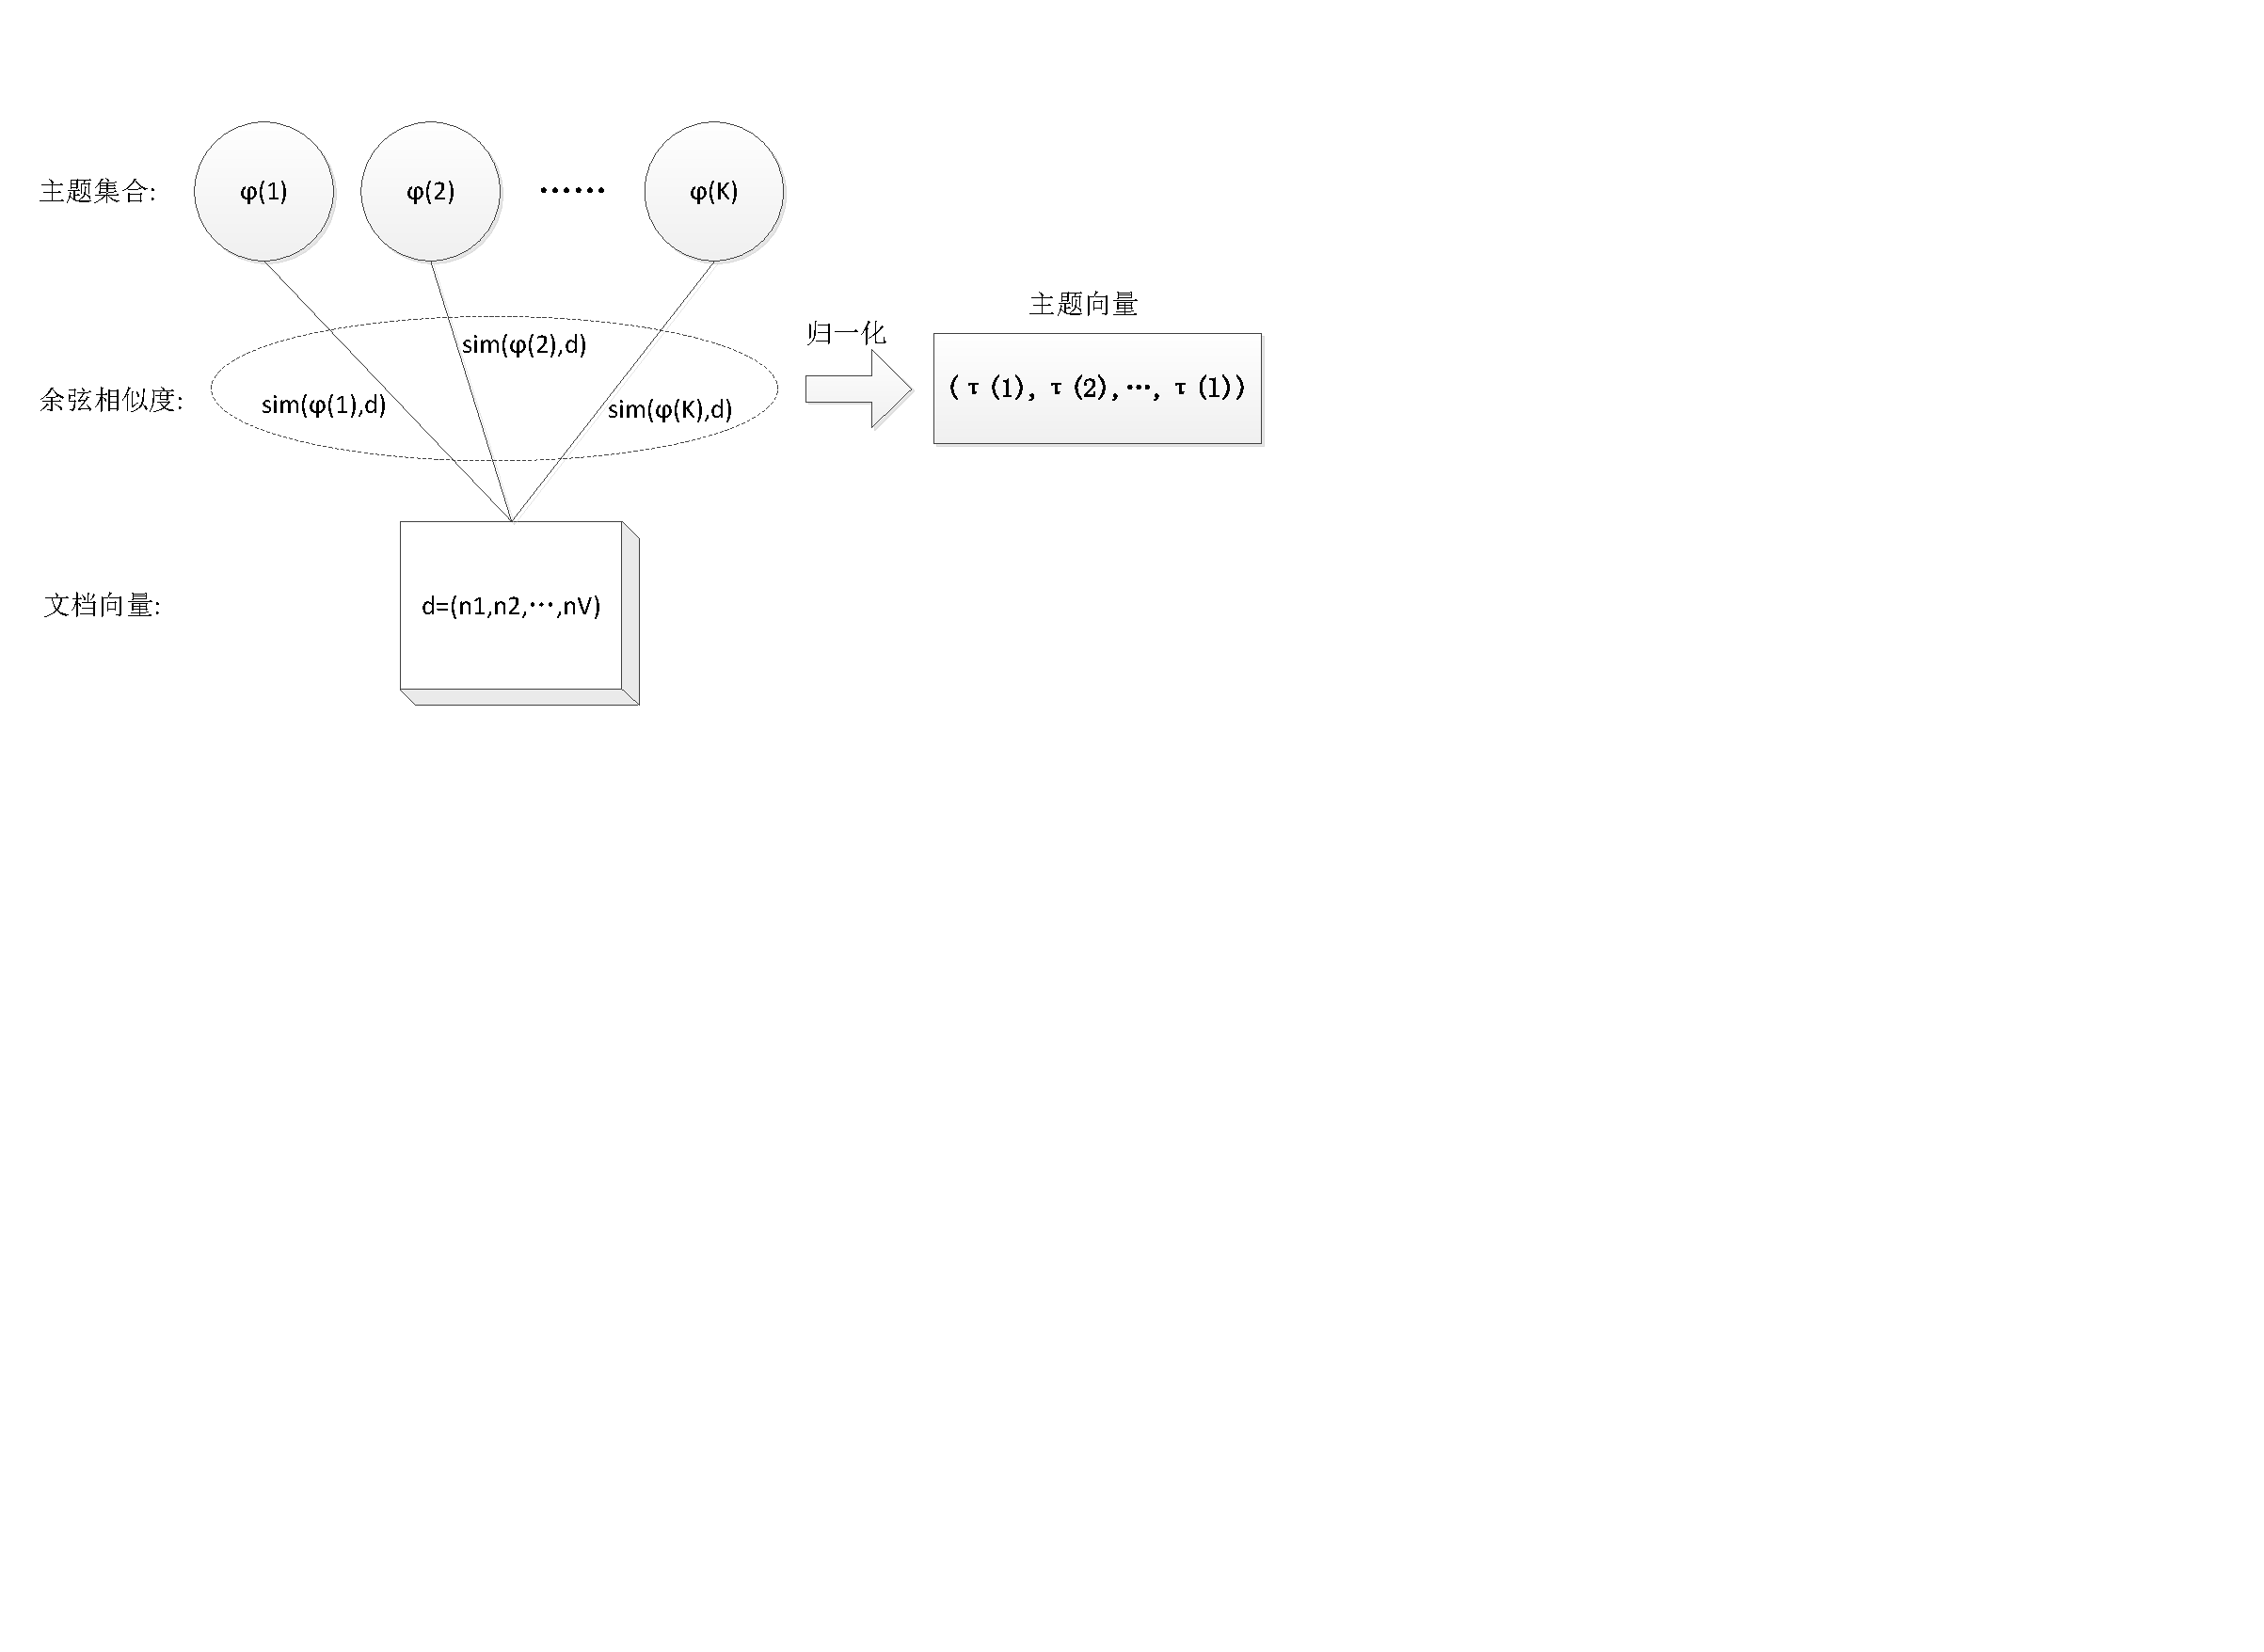
\includegraphics[width=\textwidth]{identifytopic.pdf}
\caption{基于相似度的长文本主题识别算法过程示例}
\label{fig:identifytopic}
\end{figure}

从图\ref{fig:identifytopic}中可以发现,主题集合中的$K$个主题分布$\vec{\phi_1},\vec{\phi_2},...,\vec{\phi_K}$在经过LDA推理后,其每个值得到的都是关于词汇表$V$中词汇的权重,从而组成一个$|V|$维的向量,这与文档向量$\vec{w}$的维数是一样的,当然这里的$\vec{w}=(n_1,n_2,...,n_{|V|})$,即对词汇表中每个词汇的频数(因为这里只有一篇文档,没有办法将文档向量表示成TF-IDF值)。然后通过计算主题分布于文档向量间的相似度$d_k=sim(\vec{\phi_k},\vec{w})$,得到一个新的$K$维向量,记为$\vec{s}=(d_1,d_2,...,d_K)$,但是这个向量中每个值之和并不为1,因此要进行一次归一化操作从而得到一个修正后的向量$\vec{s'}$:
\begin{equation}
  \vec{s'}=(d_1',d_2',...,d_K'),~~(d_k'=\frac{d_k}{\sum_{i=1}^{K}d_i},k\in[1,K])
\end{equation}
其中$d_k'$表示文档$d$拥有第$k$个主题的权重。然后,对$\vec{s'}$中的每个值进行从大到小的排序,排序后得到向量$\vec{s''}=(d_{k_1},d_{k_2},...,d_{k_K})$,其中$d_{k_i}$表示文档中编号为$k_i$的主题占有的权重,$i$表示该主题所占的权重在文档$d$中的重要性排在第$i$位。最后,对于给定的$\epsilon$,在$\vec{s''}$中选择前$l$个主题且满足$\sum_{i=1}^{l}d_{k_i}>\epsilon$。这时文档$d$的主题向量$\vec{\tau}$为:
\begin{equation}
  \vec{\tau}=(d_{k_1},d_{k_2},...,d_{k_l})~~(l\in[1,K])
\end{equation}

这个算法的时间复杂度是$O(K\cdot |V|)$,因为在计算主题分布和文档的相似度时,消耗的时间是$O(K\cdot |V|)$,在之后对向量权重进行排序的时候,平均时间复杂度达到$O(K\cdot log~K)$,很显然$log~K\ll|V|$,所以总共的时间复杂度是$O(K\cdot |V|)$。

\subsubsection{基于标签的主题分析技术}
对于上述提出的算法,可以基本实现对新文本进行主题标注的功能,但是上述算法存在一个很重要的问题,准确地说应该是主体模型LDA导致的一个问题。因为LDA是无监督学习,与K-mean等聚类算法相似,虽然它们可以计算出最后$K$个主题分布,但是对于每个主题分布的实际含义还需要人工标注,通过观察主题分布中的主题词来判断用什么词可以概括相应的主题。如表格\ref{tbl:topics}所示,第一行中的主题名称都是有人工标注的,这无疑造成了很大的麻烦,原因如下。
\begin{itemize}
  \item 自动化:在信息自主流动的机制中,由于主题数量巨大,主题也会不断地更新,因此用户不适合每次都使用手动标注,更好的办法是将更多的任务交给每个节点的智能系统进行处理。
  \item 歧义性:在表格中可以看到,虽然第一列标注为艺术,但是这一列的主题词也可以换成一个更加小的概念,比如电影艺术等等。同样第二列主题标注为财务,但是同样也可以认为是预算、经济等相同意义的词。
\end{itemize}

\begin{table}
\caption{主题模型训练后的主题示例}
\centering
\begin{tabular}{cccc} 
\hline
“艺术” & “财务” & “孩子” & “教育” \\
\hline
新的 & 百万 & 小伙伴 & 学校\\
电影 & 税收 & 女性 & 学生\\
展览 & 项目 & 人们 & 大学\\
音乐 & 上亿 & 多年 & 教育\\
影片 & 政府 & 家庭 & 教师\\
播放 & 每年 & 工作 & 高等\\
乐器 & 开销 & 家长 & 公开的\\
最好的 & 全新的 & 说 & 多媒体\\
演员 & 省市 & 回家 & 基础的\\
首次 & 计划 & 福利 & 试卷\\
戛纳 & 资金 & 爸爸 & 丰富的\\
剧院 & 扶植 & 比例 & 电子化\\
电影院 & 企业 & 关心 & 准时\\
爱 & 繁荣 & 生活 & 兴趣\\
票房 & 单位 & 愉快的 & 山区\\
\hline
\end{tabular}
\label{tbl:topics}
\end{table}

对于如今的互联网文本来说,文本资源其实不仅仅包含纯文本,而且还有一些元数据,其中最常见的新闻和博客资源中还包含了标签信息。因此,现在的问题是如何利用这些文本的标签的信息来重新训练主题,使得训练出来的主题都自动分配到一些标签。这里有两个问题,一个是如何通过语料库训练出带有标签的主题,另一个是如何给文档赋上多个带有标签的主题。对于第一个问题,一个比较成熟的方法是利用Labeled-LDA模型,或者L-LDA\cite{ramage2009labeled}重新训练这些主题。这里先对L-LDA模型进行简单的说明,进而对比该模型生成的主题与传统LDA生成的主题的不同之处,以及如何在下文中的进行修改使用。

L-LDA同样是一个概率图模型,其模拟了一个带有标签的文档集合的生成过程,换句话说,其充分利用了互联网上文档自带的标签数据。与LDA相同的地方是在生成过程中,每个单词依然是从一个选定的主题中生成的,但不同的是,该模型是一种有监督学习算法,通过分析标签与主题之间的对应关系来判断文档对应的标签是什么。接着前文对LDA的形式化定义,现在假设共有$K$个不同的标签对应$K$个不同的主题,完整的生成过程如下:首先从给定的参数$\vec{\beta}$的Dirichlet分布中抽样得到$K$个主题分布$\Phi=\{\vec{\phi_1},\vec{\phi_2},...,\vec{\phi_K}\}$,这一步与LDA中一样。与LDA直接从给定参数$\vec{\alpha}$的Dirichlet分布中取样得到的文档-主题分布$\Theta=\{\vec{\theta}_1,\vec{\theta}_2,...,\vec{\theta}_W\}$不同的是,在L-LDA中先要限制$\Theta$使其能与标签一一对应。于是,在这个过程中先生成文档$d$的标签$\vec{\Lambda_d}$,使其从伯努利分布中进行抽样,即
\begin{equation*}
  \vec{\Lambda_{d,k}}\in \{0,1\}\sim Bernoulli(\cdot|\Gamma_k)
\end{equation*}
其中,$\Gamma_k$是标签的先验概率。接着,定义文档的标签向量为$\vec{\lambda_d}=\{k|\Lambda_{d,k}=1\}$,从而可以为每个文档$d$定义一个$M_d\times K$维的标签映射矩阵$L_d$,其中$M_d=|\vec{\lambda_d}|$对于矩阵中的每一行$i\in \{1,...,M_d\}$和每一列$j\in \{1,...,K\}$有:
\begin{equation}
  L_{d,i,j}=\left\{
  \begin{aligned}
    1 && \mbox{if}~\lambda_{d,i}=j \\
    0 && \mbox{otherwise}
  \end{aligned}
  \right.
\end{equation}
换句话说,如果矩阵中的第$i$行在第$j$列的值是1的话只有当第$i$个文档标签$\lambda_{d,i}$等于编号为$j$的主题,否则就是0,这样就限制了主题和标签一一对应的关系。同时,这个矩阵$L_d$可以用来对Dirichlet分布中的超参数$\vec{\alpha}=(\alpha_1,\alpha_2,...,\alpha_K)^T$进行降维,得到文档$d$自己的超参数$\vec{\alpha}_d$:
\begin{equation}
  \vec{\alpha}_d=L_d\times \vec{\alpha}=(\alpha_{\lambda_{d,1}},...,\alpha_{\lambda_{d,M_d}})^T
\end{equation}
很明显可以看到,这个向量的维度原本是受主题数量决定的,现在转而由标签数量决定。在完成上面这个额外的过程后,原本的文档-主题分布$\vec{\theta}_d$可以从改进后的超参数$\vec{\alpha}_d$来取样。最后根据LDA中的生成单词方法继续执行。关于这个模型的参数训练方法不再详细赘述,推理过程将直接参照文献\cite{ramage2009labeled}中的方法。

\begin{figure}[ht]
\centering
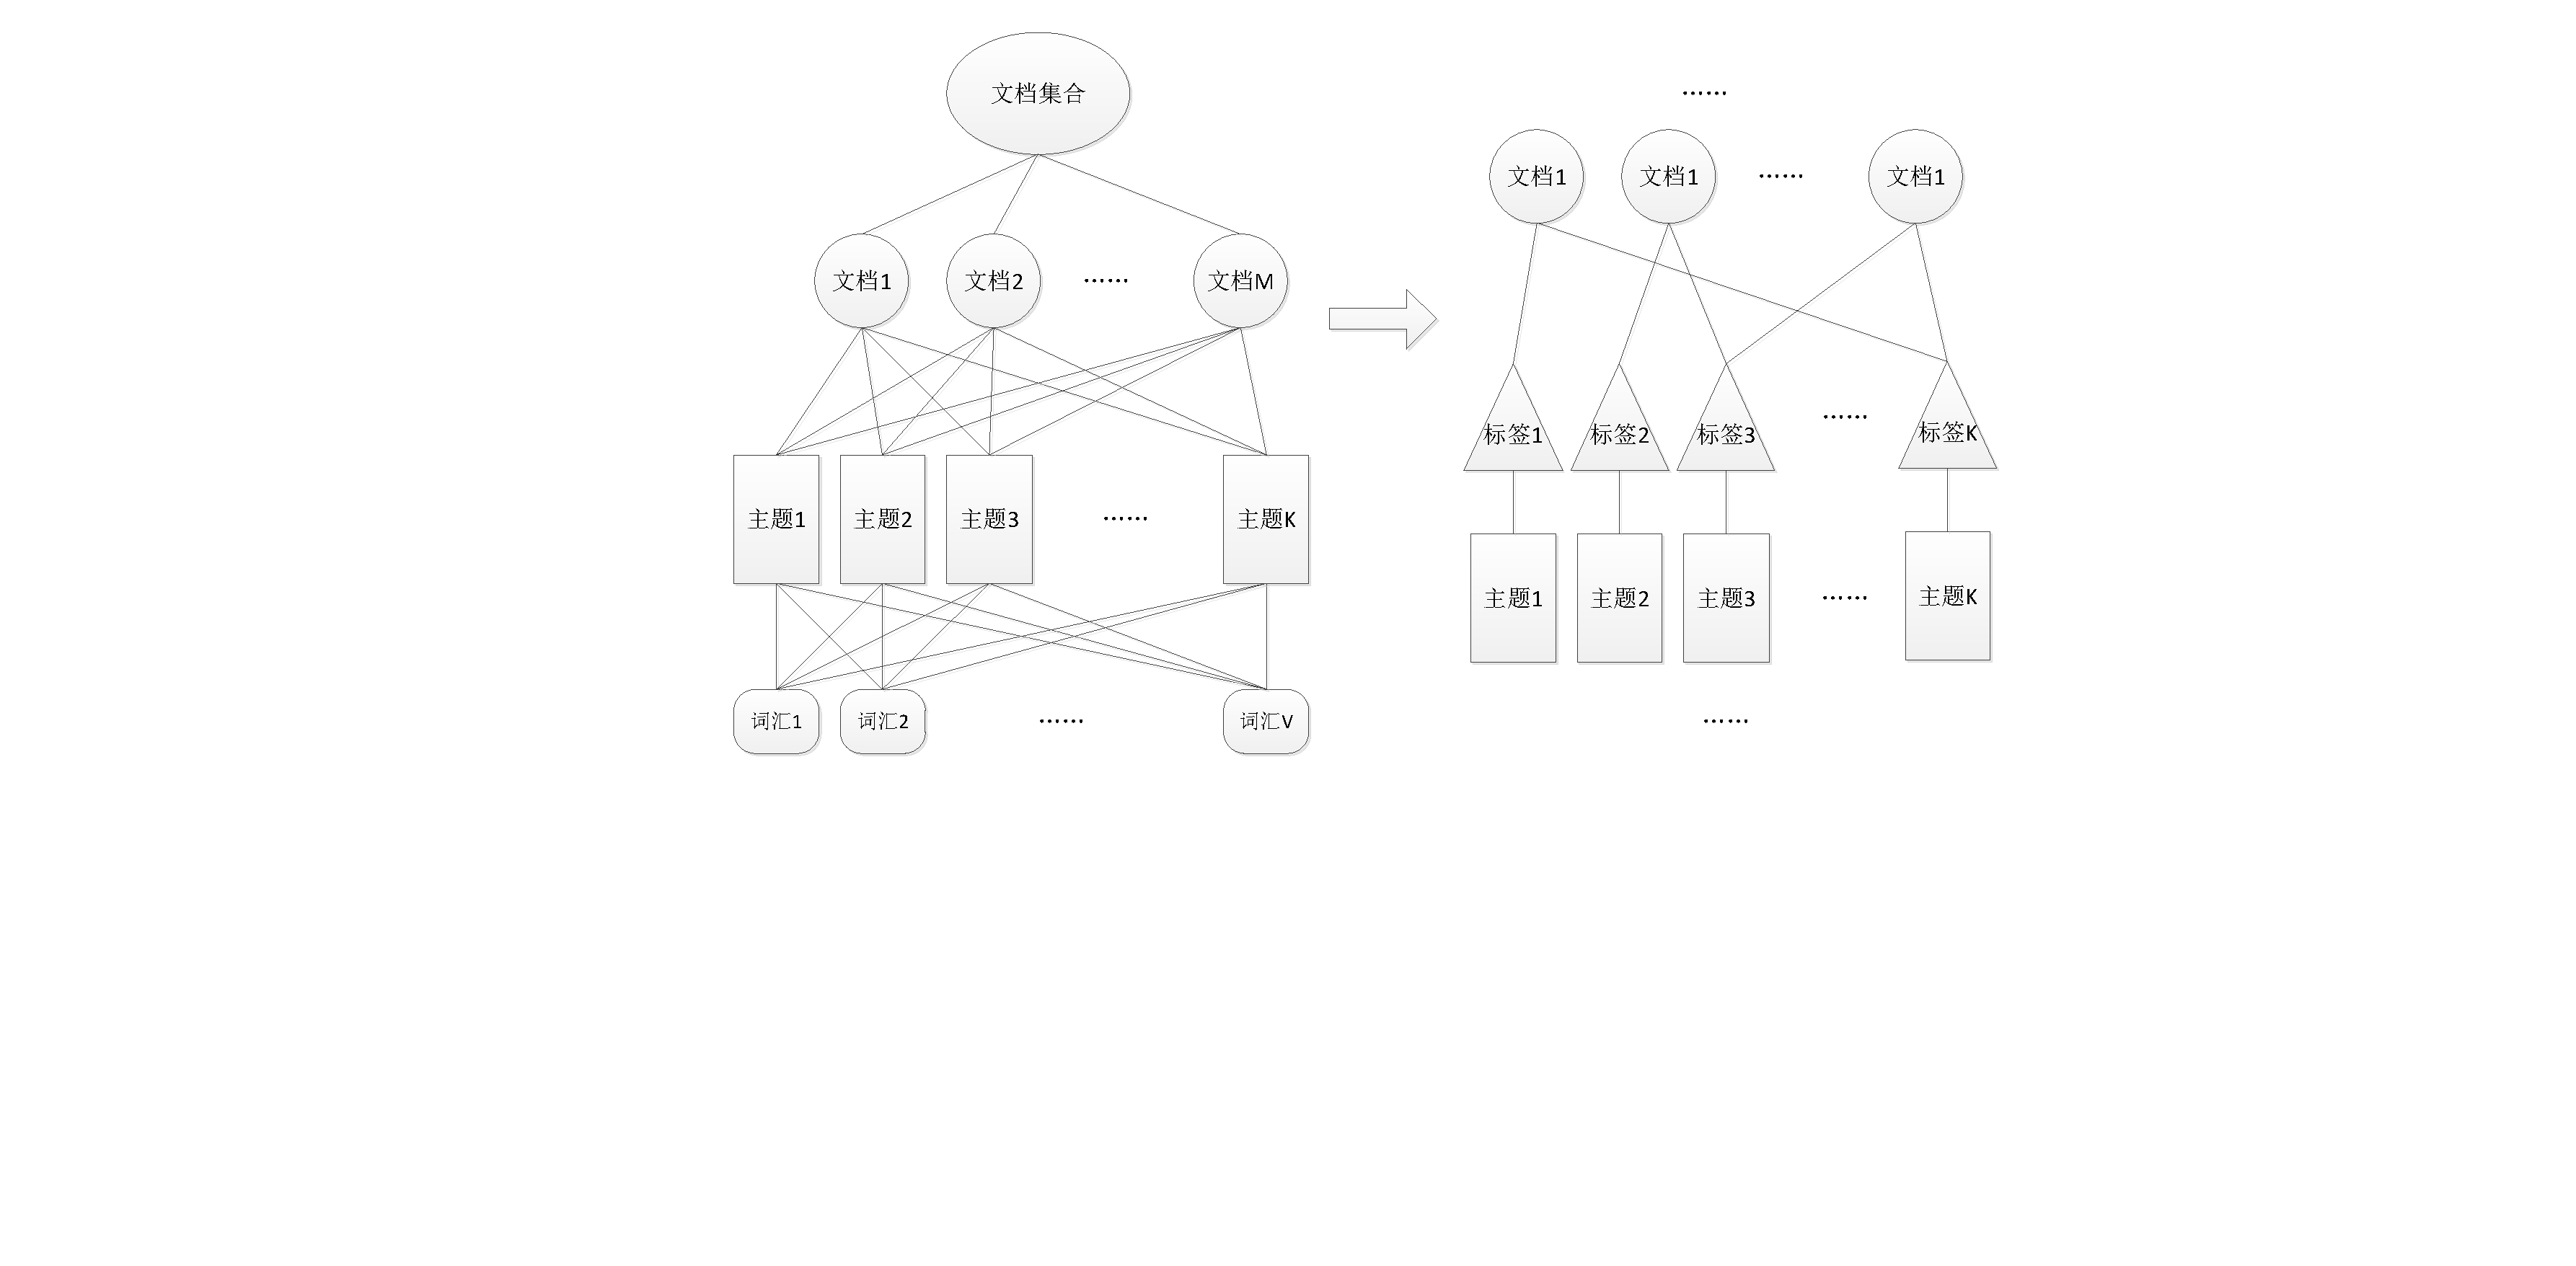
\includegraphics[width=\textwidth]{llda.pdf}
\caption{LDA模型与L-LDA模型之间的区别}
\label{fig:llda}
\end{figure}

如图\ref{fig:llda}所示,左半部分为LDA模型的层次结构,右半部分为L-LDA模型的层次结构。通过对比可以发现,两种模型的目标都是为了推理计算出主题的隐藏层,但是L-LDA比LDA多出了一层标签(中间三角形)。而这一层的目的也十分地明确,一方面是为了找到与主题一一对应的关系,弥补原本LDA无监督学习导致的主题名称不明确的问题;另一方面是在训练过程中减少了工作量,如上述公式中$\vec{\alpha}$由原本的$K$维降到了向量$\vec{\alpha}_d$的$M_d$维,因此添加标签这层导致了一个一举两得的结果。

\subsubsection{基于标签的长文本主题识别算法}
现在利用L-LDA训练出的带有标签的主题对长文本主题识别问题的算法进行修正:首先保持估计出来的主题-单词分布$\Phi$保持不变,对新文档的每个单词随机一个主题编号,然后通过Gibbs Sampling采样出每个单词新的主题编号,反复迭代直至Gibbs Sampling收敛,最后统计该文档中主题的分布$\vec{\theta}_d$,选取前$l$个主题使得它们的权重达到$\epsilon$,这样就初步推理出了文档的主题集合的一个解。随后,再按照之前基于相似度的主题识别算法中同样的步骤计算出该文档的主题集合的第二个解。通过选取两个解集合中的交集主题,并找到这些主题对应的标签,从而得到文档的标签集合。之所以计算两次主题向量并再取交集的原因是:
\begin{itemize}
  \item 文档标签数量很少:因为L-LDA模型适用于互联网上带有标签的文档,而通过统计和观察,这些文档的平均标签数相对于主题的数量是十分少的,只有2-3个。但是,在第一个主题识别算法中,主题选取的数量依赖于给定的阈值$\epsilon$,当$\epsilon$达到95\%的时候,根据普通LDA对文本数据集的实验结果来看,每个文档会7-8个主题,因此是不符合实际情况的。通过去交集的办法可以过滤掉一些可能是噪声的主题。
  \item 主题数量的不确定性:因为在两个模型中,主题数量$K$都是人工确定给定,因此$K$的大小会间接决定了文档最后的标签数量。而L-LDA是根据已有文档的标签集合进行有监督的学习,因此在控制每个文档的标签数量上更加出色。
\end{itemize}

\subsection{短文本信息的分析与建模方法}
互联网中的短文本一般包括各种资源的评论、微博的内容,甚至是资源的元数据,针对这些数据的分析目前已经有比较的研究,在此就不再罗列。本节要研究的短文本信息是一种新型出现的视频弹幕,考虑到这种弹幕数据独有的特性,因此可以用来对视频精彩片段进行提取和索引。相比于利用图像技术进行视频精彩镜头提取的工作,利用弹幕短文本来做的优势是:
\begin{enumerate}
  \item 图像本身很难被计算机充分理解,因为视频中讲述的故事很难用像素点来表示,计算机不像人类一样可以通过图像描述的方式来理解这些隐藏的主题。
  \item 当用户对视频进行查询时,一般是通过输入文本信息的,因为这是一种简单而有效的交互方式,所以这不可避免需要进行文本和图像之间的转换。虽然现在已经有技术来实现这一功能,但是相比文本的匹配过程,这种技术显然是更加耗时耗资源的。
\end{enumerate}

基于上述理由,一种更好的方式是利用弹幕这种带有时间戳的短文本对视频的精彩镜头进行描述。这节的研究成果所发表的论文已经被ACM MobiHoc 2015 - HotPOST '15录用,其中MobiHoc是CCF推荐的B类会议,HotPOST是其下的一个workshop。在这一节中,将简单说明该论文的内容。

\subsubsection{视频精彩镜头的抽取问题}
为了简化问题,假设弹幕的文本内容可以充分用一个关键词来表示,关键词来自一个充满情感词的词典,这样做的理由是:
\begin{itemize}
  \item 直观上来看,每个用户在看完一个精彩镜头之后都会触发最多一种情感,所以弹幕的内容应该是单一的。比如看完一个恐怖镜头之后,人可能会感到恐惧。
  \item 统计上来说,弹幕是典型的短文本,在本文的数据集中平均只有6.28个中文字符。
\end{itemize}

首先来形式化定义一下待解决的问题。一个时间长度为$T_v$秒的视频$v$可以被分割成一个连续小段的序列,$v={f_{v,1},f_{v,2},...,f_{v,N_v}}$,其中小段$f_{v,i}~(1\le i\le N_v)$的时间长度是固定的$T_f$,比如是256毫秒。显然,视频$v$中小段的数量$N_v=T_v/T_f$,其中最后一个小段可能比$T_f$短。类似的,精彩镜头$s_v$也是视频$v$中的一个连续子序列,记作$s_v=\{f_{v,i}, f_{v,i+1}, ..., f_{v,j}\}~~(1\le i\le j\le N_v)$。基于之前的假设,本文的的弹幕表示成三元组$c_{v,i}=(w, t_0, T_c)$,其中$w_k$是来自词典$\mathcal{W}$的情感词,$t_0$是弹幕在视频$v$中的开始时间戳,$T_c$是弹幕出现在屏幕上的持续时间,每个视频的弹幕集合通常包括了很多不同的关键词和开始时间戳。对于视频$v$中的弹幕集合记为$\vec{c_v}=\{c_{v,1}, c_{v,2},..., c_{v,M_v}\}$。所有符号见表\ref{tbl:notation}所示,精彩镜头、视频小段和弹幕的关系如图\ref{fig:tscrelation}所示。

\begin{table}
\caption{本模型中用到的符号}
\centering
\begin{tabular}{c c} 
\hline
SYMBOL & DESCRIPTION \\ 
\hline
$v$ & time-sync commented video \\
$T_v$ & video length (time duration) \\
$N_v$ & total number of frames in video $v$ \\
$f_{v,i}$ & $i$-th frame in video $v$ \\
$T_f$ & frame length (time span) \\
$s_v$ & highlight shot in video $v$ \\
$c_{v,i}$ & $i$-th TSC in video $v$ \\
$w$ & sentimental keyword of TSC \\
$t_0$ & start time stamp of TSC \\
$T_c$ & TSC length (time span) \\
$M_v$ & total number of TSCs in video $v$ \\
$e_v$ & global emotional feature of video $v$ \\
$\mathcal{V}$ & video corpora of size $|\mathcal{V}|$ \\
$\mathcal{C}$ & TSC corpora of size $|\mathcal{V}|$ \\
$\mathcal{W}$ & sentimental keywords dictionary of size $|\mathcal{W}|$\\
\hline
\end{tabular}
\label{tbl:notation}
\end{table}

\begin{figure}
\centering
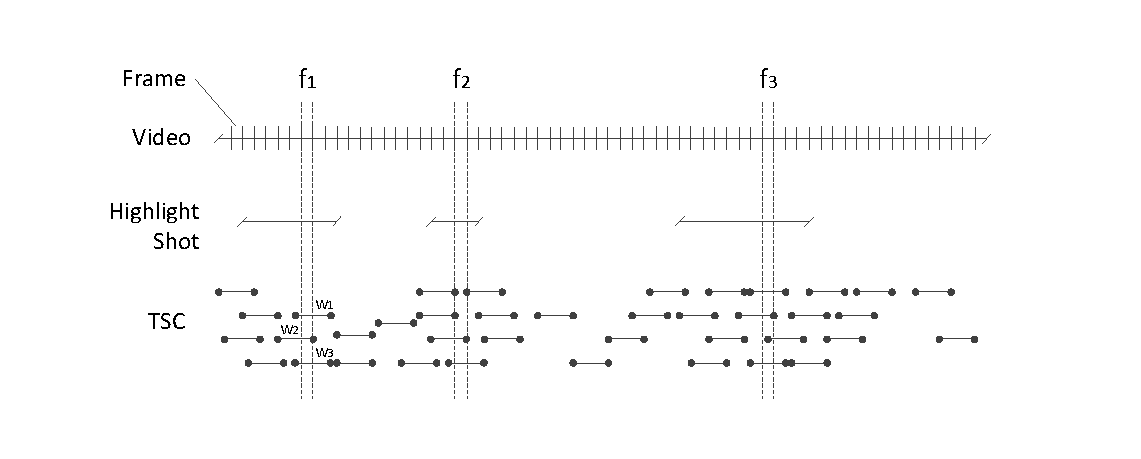
\includegraphics[width=\textwidth]{tscrelation.pdf}
\caption{视频、小段、镜头和弹幕之间的关系}
\label{fig:tscrelation}
\end{figure}

下文将主要关注视频的精彩镜头抽取和查询的过程,问题定义如下:
\begin{mydef}[视频精彩镜头的抽取问题]
  给定视频$v$和其弹幕集合$\vec{c_v}$,求出可能的精彩镜头集合$\vec{s_v}=\{s_{v,1}, s_{v,2},...\}$,且任何两个$s_{v,i}$和$s_{v,j}$是不相交的。
\end{mydef}
\begin{mydef}[视频精彩镜头的查询问题] 
  给定查询的精彩镜头$s_q$、视频$v$和对应的弹幕$\vec{c_v}$,求出视频$v$中的具有相似情感的精彩镜头。
\end{mydef}
为了解决上述两个问题,我们需要做的是:
\begin{enumerate}
  \item 如何利用弹幕来描述小段、镜头和视频;
  \item 如何计算小段与小段、镜头与镜头之间的相似度;
  \item 如何自动发现精彩镜头的边界;
\end{enumerate}

\subsubsection{弹幕短文本的特征}
对弹幕这种短文本的特征进行研究有助于计算视频小段间的相似度。因为弹幕之前被定义成一个三元组$c=(w, t_0, T_c)$,假设关键词$w$已经从现有成熟的技术从原始评论文本转换来的。经验上,用户只有当他被当前或者临近的前几个镜头所感染,这说明了弹幕只是在时间段$[t_0, t_0+T_c]$的开头更加有效。所以,这里提出了一种弹幕强度在时间段$[t_0, t_0+T_c]$上的衰退函数$g_c$:
\begin{equation}
  g_c(t)=
  \begin{cases}
    T_c^{t_0-t}, & \text{if } t_0\le t\le t_0+T_c \\
    0, & \text{otherwise}
  \end{cases}
\label{eq:strength}
\end{equation}
可以看到,弹幕在$t_0$的时候强度最大,在之后的$T_c$秒内,强度逐渐趋向于0,这解释了弹幕在不同时间戳的时候是如何反应用户情感的。

\subsubsection{视频小段的表示和相似度}
如图\ref{fig:tscrelation}表示,每个小段都或多或少包含了一些弹幕,所以最简单的方式来描述小段是用一个关于关键词词频的向量$f=(n_1, n_2,..., n_{|\mathcal{W}|})$,其中$n_i(1\le i\le |\mathcal{W}|)$是词典中第$i$个关键词在小段中出现的数量。举例来说,在小段$f_1$的区间上,有三个关键词$w1$、$w2$和$w3$,因此$f_1=(1, 1, 1, 0, 0, ...)$。Jaccard相似度可以用于计算小段之间的相似程度,但是当两个小段中的关键词都是同义词时,就不适用了。根据弹幕强度衰退函数来看,关键词的强度是一个更好的选择,另一方面,弹幕在每个视频小段内的数量都远小于$M_v$,因此会导致小段的歧义性。

所以,在时刻$t$,小段$f_v=(g_1, g_2,..., g_{|\mathcal{W}|})$中的关键词强度向量可以计算为:
\begin{equation}
  g_i=\sum_{c\in\vec{c_f}}g_c(t)
\label{eq:framestr}
\end{equation}
其中 $\vec{c_f}$是视频$v$的弹幕的集合:
\begin{equation*}
  \vec{c_f}=\{c|w=w_i, t-T_c<t_0<t+T_f \}
\end{equation*}
图\ref{fig:framestr}解释了弹幕关键词关于小段的表示方式。

\begin{figure}
\centering
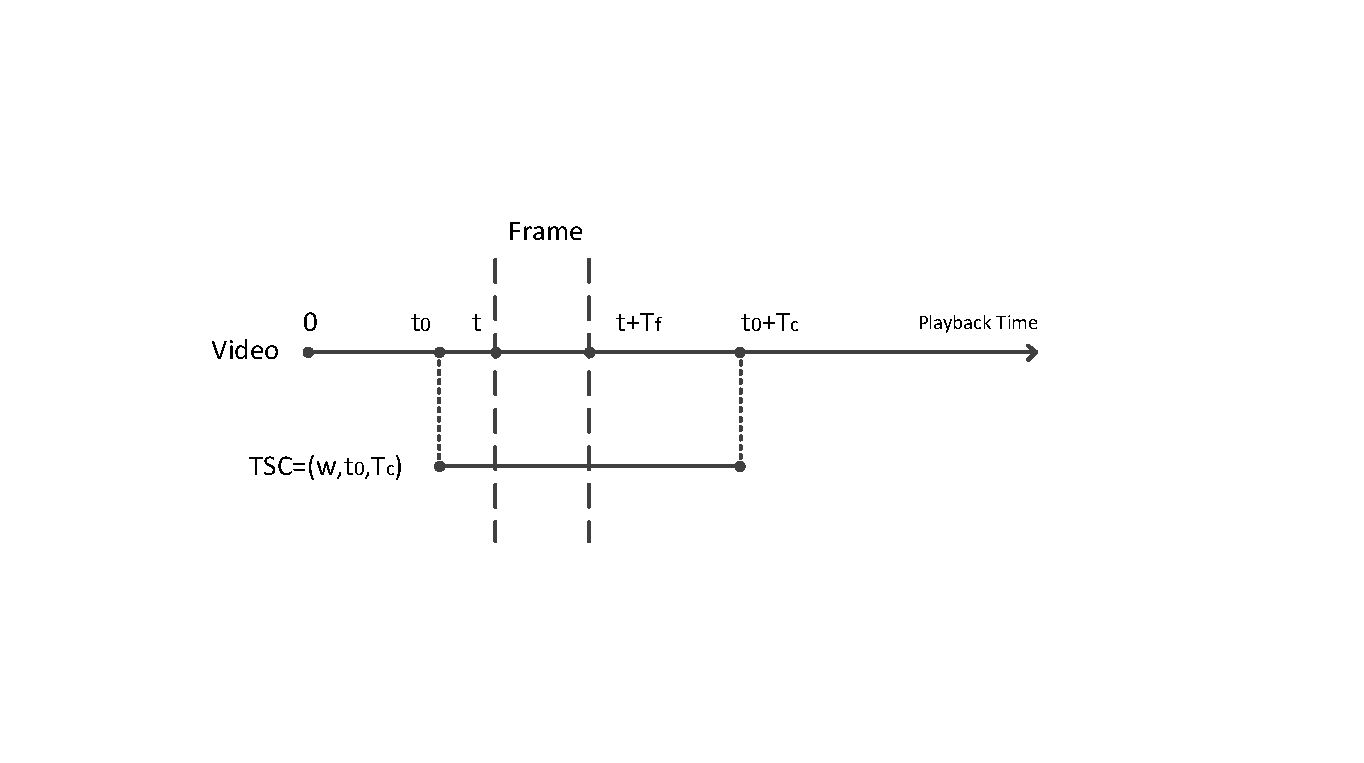
\includegraphics[width=0.8\textwidth]{framestr.pdf}
\caption{对于关键词强度向量的每一维度,找出所有的弹幕使得其时间区间与小段的时间区间相交}
\label{fig:framestr}
\end{figure}

但是,利用视频小段的关键词强度向量来计算Jaccard相似度仍然有不足,因为每个小段的弹幕数量是十分有限的。为了解决这个问题,引入一个新的变量$e_v$,称为视频$v$的全局情感特征。在实际的例子中,全局情感特征与用户在看完一个精彩镜头之后抒发的情感是一致的。同时,精彩镜头中的局部情感特征在一定程度上组成了全局情感特征,而且精彩镜头和视频都是由小段组成的。鉴于此原因,特征相似度的计算在小段和全局情感特征间进行,而不是小段间的相似度。

为了获得视频$v$的全局情感特征,这里使用了传统的LDA主题模型。原本文本中的文档-主题-词汇三层关系转换成了视频-特征-弹幕的关系,其中弹幕中的关键词与单词是类似的。另一方面,这里的视频仅仅考虑文本信息,而排出了图像信息,所以它可以表示为一个带有权重的全局情感向量。类似于文档的主题,全局情感特征是一个隐藏变量,并定义为关于关键词的分布,$e_v=(n_1, n_2,...,n_{|\mathcal{W}|})$,为了简化问题,假设总共只有$K$个不同的特征。

在应用LDA之前,弹幕生成的过程与文档的生成过程有两个小区别:
\begin{itemize}
\item 精彩镜头的影响:精彩镜头是视频中额外的特殊元素,而在文件中没有完全相同的概念。正如前文所说,弹幕的主要是受精彩镜头影响,更具体地来说,是局部情感特征。为了简化问题,这里特意把弹幕的生成,通过大体上,由视频,即全局情感特征的影响。在实验中,我们表明,这种近似计算还执行比其他传统的方法要好得多。
\item 弹幕密度影响:弹幕的密度反映了弹幕视频的特征,因为一些现有的工作使用频率提取镜头。不同于文档,其中的每一个单词是依次产生并均匀地分布的,而弹幕生成的不确定性取决于用户的感觉是否将被某个镜头所触发。例如,弹幕更可能在精彩镜头的区间内生成。 
\end{itemize}

现在,可以开始衡量小段和全局情感特征之间的相似性。鉴于视频集合$\mathcal{V}=\{v_1, v_2,..., v_{|\mathcal{V}|}\}$,而弹幕集合$\mathcal{C}=\{\vec{c_{v_1}}\}$,其中的关键字来自大小为$|\mathcal{W}|$的字典,可以得到大小为$|\mathcal{V}|$*$|\mathcal{W}|$的视频-弹幕矩阵,矩阵元素的值是关键字的数量。为了分解的视频-弹幕矩阵成两个矩阵,大小为$|\mathcal{V}|$*$K$的视频-特征矩阵和大小为$K$*$|\mathcal{W}|$的特征-弹幕矩阵。在这种情况下应用的时LDA,而不是SVD,因为LDA在主题分析上更好,尽管其速度推理过程比SVD要慢一点。在此之后,我们可以得到小段$f_v$的特征相似度$d_f$,通过$f_v$的关键字强度向量和全局情感特征之间$ e_v$:
\begin{equation}
d_{f_v}=cos(f_v,e_v)=\frac{\sum_{i=1}^{|\mathcal{W}|}g_i \times n_i}{%
\sqrt{\sum(g_i)^2} \times \sqrt{\sum(n_i)^2}}
\end{equation}

\subsubsection{精彩镜头边界检测}
之后,根据给定的全局情感特征,得到特征相似度$d_f$,就可以通过算法\ref{alg:highlight}检测出精彩镜头的范围。该算法表明,在每次迭代期间,小段的最大的特征相似度在全局情感特征中是第一次被选出的,并且从中间向两侧依次比较。此外,还需要设置两个阈值。 $\epsilon$控制了下边界的最大相似特征$d_{f_{v,k}}$,这是因为如果$d_{f{v,k}}$过小,可能没有具有这种情感的精彩镜头存在,所以应该忽略这个特征。 $\delta$ 控制了潜在的精彩镜头的最左边和最右边小段的边界。更好的方法是根据不同的视频,设置动态的$\delta$ ,因为阈值会随着弹幕的数量和视频的长度变化。
\begin{algorithm}
\caption{精彩镜头的边界检测算法}
\ForEach{frame $f_{v,i} \in v$}{
   calculate keyword strength vector $f_{v,i}=(g_1, g_2,..., g_{|\mathcal{W}|})$\;
}
\ForEach{global emotional feature $e_{v,j} \in e_v$}{
  \ForEach{each frame $f_{v,i} \in v$}{
    calculate feature similarity $d_{f_{v,i}}=cos(f_{v,i}, e_{v,j})$\;
  }
  find $max(d_{f_{v,k}})$ indexed by $k$\;
  \lIf{$d_{f_{v,k}} < \epsilon$}{continue}
  set $n_l:=k-1$\;
  \lWhile{$n_l \ge 1$ and $|d_{f_{v,n_l}}-d_{f_{v,n_l+1}}|<\delta$}{$n_l:=n_l-1$}
  set $n_r:=k+1$\;
  \lWhile{$n_r \le N_v$ and $|d_{f_{v,n_r}}-d_{f_{v,n_r-1}}|<\delta$}{$n_r:=n_r+1$}
  $\{f_{v,n_l},...,f_{v,n_r}\}$ is the highlight shot with feature $e_{v,j}$\;
}
\label{alg:highlight}
\end{algorithm}

\subsubsection{精彩镜头相似度计算}
一旦精彩镜头从视频提取出来之后,就可以计算出该精彩镜头的局部特征向量$\vec{e_s}=(w_1, w_2,..., w_K)$,其中每个$w_i$是精彩镜头$s$的每一个特征维度的权重。首先,计算出精彩镜头的关键词词频$n_s=(n_1, n_2,..., n_{|\mathcal{W}|})$。然后,对每一个视频的全局情感向量的特征$e_{v,k}=(n_1, n_2,...,n_{|\mathcal{W}|})$和权重$w_{v,k}$,计算余弦相似度:
\begin{equation}
  w_k=w_{v,k}\times cos(n_s, e_{v,i}), (1\le k\le K)
\end{equation}
然后,对给定的两个精彩镜头,各自计算它们的局部特征向量$\vec{e_{s_1}}$和$\vec{e_{s_2}}$之后,就可以衡量它们之间在语义上的相似度了。

\subsection{文本网的分析与建模方法}

\subsection{文本流的分析与建模方法}

\subsection{小结}
